\documentclass{article}
\usepackage[utf8]{inputenc}
\usepackage[T1]{fontenc}
\usepackage{listings}
\usepackage{color}
\usepackage{graphicx}
\usepackage{fontspec}
\usepackage[pdftex]{hyperref}
\setlength{\parindent}{0pt}

% YAML code color settings for listings package
\definecolor{gray}{rgb}{0.5,0.5,0.5}
\definecolor{orange}{rgb}{1,0.5,0}
\lstset{
    language=bash,
    basicstyle=\ttfamily,
    keywordstyle=\color{blue},
    commentstyle=\color{gray},
    stringstyle=\color{orange},
    breaklines=true,
    breakatwhitespace=true,
    showstringspaces=false
}


\title{Zarządzanie Systemami Rozproszonymi\\Laboratoria z Service Mesg i Istio}
\author{mgr inż. Jakub Woźniak}
\date{}

\begin{document}

\maketitle
\section{Wprowadzenie}

\subsection{Co to jest Service Mesh?}

Service Mesh to dedykowana warstwa infrastruktury, która zarządza komunikacją między mikroserwisami w aplikacjach rozproszonych. Umożliwia dodanie zaawansowanych funkcji bez modyfikacji kodu aplikacji.

\textbf{Podstawowe funkcje Service Mesh:}
\begin{itemize}
    \item \textbf{Routing ruchu:} Określanie, jak ruch sieciowy jest kierowany między mikroserwisami.
    \item \textbf{Obserwowalność:} Zbieranie metryk, logów i tras przepływu ruchu w aplikacjach.
    \item \textbf{Bezpieczeństwo:} Szyfrowanie ruchu między usługami (TLS), autoryzacja i uwierzytelnianie.
    \item \textbf{Zarządzanie błędami:} Mechanizmy takie jak \textit{Circuit Breaking} i \textit{Fault Injection}, które zwiększają odporność systemu na awarie.
\end{itemize}

\subsection{Dlaczego Service Mesh jest potrzebny?}

W tradycyjnych monolitycznych aplikacjach komunikacja wewnętrzna była zarządzana w obrębie jednego procesu. W przypadku aplikacji mikroserwisowych, które działają jako niezależne komponenty, komunikacja między nimi wymaga zaawansowanego zarządzania.

\textbf{Korzyści z Service Mesh:}
\begin{itemize}
    \item \textbf{Spójność:} Ujednolicone zarządzanie ruchem między usługami.
    \item \textbf{Niezależność:} Funkcje takie jak routing czy bezpieczeństwo są niezależne od kodu aplikacji.
    \item \textbf{Skalowalność:} Automatyczne równoważenie obciążenia oraz optymalizacja ruchu.
    \item \textbf{Odporność:} Mechanizmy zapewniające stabilność systemu w przypadku awarii części usług.
\end{itemize}

\subsection{Wprowadzenie do Istio}

Istio to jedno z najpopularniejszych narzędzi implementujących Service Mesh. Jest w pełni zgodne z Kubernetes i zapewnia zaawansowane funkcje zarządzania komunikacją między usługami.

\textbf{Główne komponenty Istio:}
\begin{itemize}
    \item \textbf{Pilot:} Zarządza konfiguracją ruchu w klastrze.
    \item \textbf{Envoy:} Proxy działające w każdej usłudze, obsługujące ruch między mikroserwisami.
    \item \textbf{Mixer:} Zbieranie metryk i egzekwowanie polityk.
    \item \textbf{Citadel:} Obsługa uwierzytelniania i autoryzacji (m.in. TLS).
    \item \textbf{Ingress/Egress Gateway:} Zarządzanie ruchem przychodzącym i wychodzącym z klastra.
\end{itemize}

\subsection{Architektura Istio}

Architektura Istio opiera się na modelu proxy-sidecar, gdzie każda usługa w klastrze ma dedykowany proxy (Envoy) do obsługi ruchu.

\textbf{Kluczowe elementy architektury:}
\begin{itemize}
    \item \textbf{Data Plane:} Odpowiada za ruch sieciowy między usługami. Składa się z proxy Envoy wstrzykniętych jako \textit{sidecar} w każdym Podzie.
    \item \textbf{Control Plane:} Zarządza konfiguracją Data Plane oraz politykami ruchu i bezpieczeństwa.
\end{itemize}

\begin{figure}[h]
    \centering
    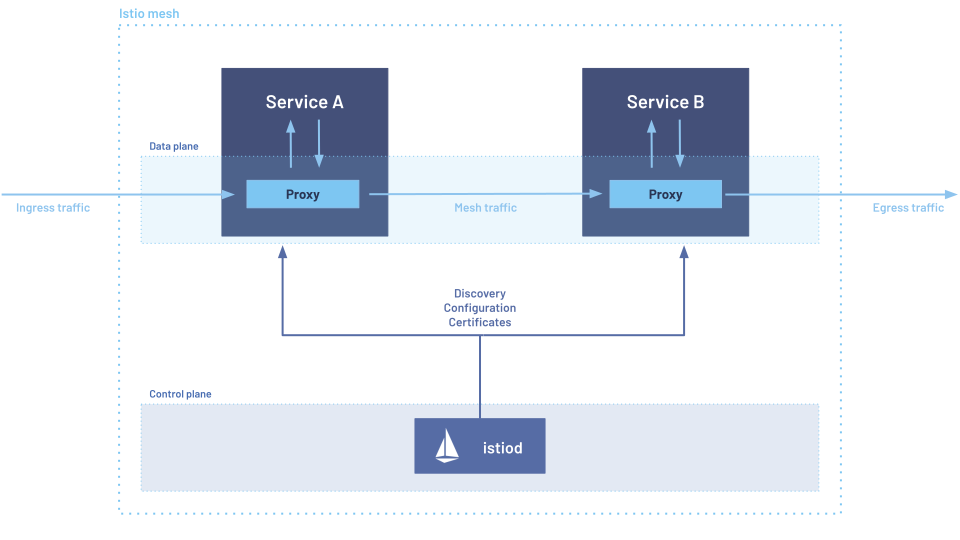
\includegraphics[width=0.8\textwidth]{resources/istio_architecture.png}
    \caption{Architektura Istio. Źródło: dokumentacja Istio.}
\end{figure}

Istio ułatwia zarządzanie złożonymi systemami mikroserwisowymi, zapewniając niezbędne funkcje do skalowalnych, bezpiecznych i wydajnych wdrożeń aplikacji w środowiskach produkcyjnych.

\section{Przygotowanie środowiska}

W tej sekcji studenci przygotują środowisko do pracy z Istio, instalując wymagane narzędzia oraz konfigurując klaster Minikube.

\subsection{Wymagane narzędzia}

Przed rozpoczęciem ćwiczeń należy upewnić się, że na komputerze są zainstalowane następujące narzędzia:
\begin{itemize}
    \item \textbf{Minikube:} Klaster Kubernetes działający lokalnie. Instalację Minikube można przeprowadzić zgodnie z oficjalną dokumentacją: \url{https://minikube.sigs.k8s.io/docs/start/}.
    \item \textbf{kubectl:} Narzędzie CLI do zarządzania klastrem Kubernetes. Instrukcje instalacji znajdują się na stronie: \url{https://kubernetes.io/docs/tasks/tools/install-kubectl/}.
    \item \textbf{Istio CLI:} Narzędzie do instalacji i zarządzania Istio. Można je pobrać poleceniem:
    \begin{lstlisting}
    curl -L https://istio.io/downloadIstio | sh -
    cd istio-<version>
    export PATH=$PWD/bin:$PATH
    \end{lstlisting}
\end{itemize}

\subsection{Instalacja Istio}

\textbf{Kroki:}
\begin{enumerate}
    \item \textbf{Uruchom klaster Minikube:}
    \begin{lstlisting}
    minikube start --cpus=4 --memory=8192
    \end{lstlisting}
    Upewnij się, że klaster jest gotowy:
    \begin{lstlisting}
    kubectl get nodes
    \end{lstlisting}

    \item \textbf{Zainstaluj Istio z profilem demo:}
    \begin{lstlisting}
    istioctl install --set profile=demo -y
    \end{lstlisting}
    Profil demo zawiera wszystkie podstawowe komponenty Istio, takie jak Ingress Gateway, Prometheus, Grafana i Kiali.

    \item \textbf{Zweryfikuj instalację Istio:}
    \begin{lstlisting}
    kubectl get pods -n istio-system
    \end{lstlisting}
    Upewnij się, że wszystkie Pody w namespace \texttt{istio-system} mają status \texttt{Running}.

    \item \textbf{Włącz wstrzykiwanie sidecarów:}
    Oznacz namespace \texttt{default}, aby Istio automatycznie wstrzykiwało proxy Envoy do nowych Podów:
    \begin{lstlisting}
    kubectl label namespace default istio-injection=enabled
    \end{lstlisting}
\end{enumerate}

\subsection{Testowanie instalacji}

Aby upewnić się, że Istio działa poprawnie:
\begin{enumerate}
    \item \textbf{Przejdź do interfejsu Kiali:}
    \begin{lstlisting}
    kubectl -n istio-system port-forward svc/kiali 20001:20001
    \end{lstlisting}
    Otwórz przeglądarkę i przejdź pod adres \texttt{http://localhost:20001}.
    \item \textbf{Przejdź do interfejsu Grafana:}
    \begin{lstlisting}
    kubectl -n istio-system port-forward svc/grafana 3000:3000
    \end{lstlisting}
    Otwórz przeglądarkę i przejdź pod adres \texttt{http://localhost:3000}.
\end{enumerate}

Po wykonaniu powyższych kroków środowisko jest gotowe do pracy z Istio i ćwiczeń na aplikacji Bookinfo.

\section{Wdrożenie aplikacji Bookinfo}

Aplikacja Bookinfo jest przykładem aplikacji mikroserwisowej, która pozwala na demonstrację funkcji Istio, takich jak routing ruchu, monitorowanie i fault injection. Składa się z czterech głównych usług: \texttt{productpage}, \texttt{details}, \texttt{reviews} oraz \texttt{ratings}.

\subsection{Architektura aplikacji Bookinfo}

\textbf{Komponenty aplikacji:}
\begin{itemize}
    \item \textbf{productpage:} Frontend aplikacji wyświetlający szczegóły produktu.
    \item \textbf{details:} Usługa dostarczająca szczegóły produktu.
    \item \textbf{reviews:} Usługa obsługująca recenzje produktu. Istnieją trzy wersje:
    \begin{itemize}
        \item \textbf{v1:} Wyświetla tylko tekst recenzji.
        \item \textbf{v2:} Wyświetla tekst recenzji z oceną liczbową.
        \item \textbf{v3:} Wyświetla tekst recenzji z oceną liczbową oraz gwiazdkami.
    \end{itemize}
    \item \textbf{ratings:} Usługa obsługująca oceny liczbowe.
\end{itemize}

Architektura aplikacji Bookinfo jest idealnym przykładem rozproszonego systemu mikroserwisowego, umożliwiającym testowanie różnych scenariuszy w środowisku Istio.

\subsection{Wdrożenie aplikacji Bookinfo}

\textbf{Kroki:}
\begin{enumerate}
    \item \textbf{Zastosuj manifesty aplikacji Bookinfo:}
    \begin{lstlisting}
    kubectl apply -f samples/bookinfo/platform/kube/bookinfo.yaml
    \end{lstlisting}
    Manifest \texttt{bookinfo.yaml} zawiera definicje Deployment oraz Service dla wszystkich komponentów aplikacji.

    \item \textbf{Sprawdź status wdrożenia:}
    \begin{lstlisting}
    kubectl get pods
    kubectl get services
    \end{lstlisting}
    Upewnij się, że wszystkie Pody i usługi są uruchomione.

    \item \textbf{Eksponuj aplikację za pomocą Istio Gateway:}
    Zastosuj manifest gateway dla Bookinfo:
    \begin{lstlisting}
    kubectl apply -f samples/bookinfo/networking/bookinfo-gateway.yaml
    \end{lstlisting}
    Gateway Istio umożliwia dostęp do aplikacji spoza klastra Kubernetes.

    \item \textbf{Znajdź adres Ingress Gateway:}
    Sprawdź adres i port \texttt{EXTERNAL-IP} dla gateway:
    \begin{lstlisting}
    kubectl get svc istio-ingressgateway -n istio-system
    \end{lstlisting}

    \item \textbf{Uzyskaj dostęp do aplikacji:}
    Przejdź w przeglądarce pod adres:
    \begin{lstlisting}
    http://<EXTERNAL-IP>/productpage
    \end{lstlisting}
\end{enumerate}

\subsection{Obserwacja ruchu w Kiali}

\textbf{Kroki:}
\begin{enumerate}
    \item Uruchom interfejs Kiali:
    \begin{lstlisting}
    kubectl -n istio-system port-forward svc/kiali 20001:20001
    \end{lstlisting}
    Przejdź pod adres \texttt{http://localhost:20001} w przeglądarce.

    \item Sprawdź przepływ ruchu między usługami:
    \begin{itemize}
        \item W Kiali wybierz namespace \texttt{default}.
        \item Obserwuj graficzną reprezentację przepływu ruchu między komponentami aplikacji Bookinfo.
    \end{itemize}
\end{enumerate}

\subsection{Podsumowanie sekcji}

Po wdrożeniu aplikacji Bookinfo studenci powinni być w stanie:
\begin{itemize}
    \item Zrozumieć architekturę aplikacji mikroserwisowej.
    \item Eksponować aplikacje przy użyciu Istio Gateway.
    \item Obserwować przepływ ruchu między usługami w narzędziu Kiali.
\end{itemize}

\section{Routing ruchu i kontrola przepływu}

Routing ruchu w Istio pozwala na precyzyjne kontrolowanie, jak ruch sieciowy jest kierowany między usługami. Dzięki regułom routingu można np. rozdzielać ruch na różne wersje aplikacji, wprowadzać ważenie ruchu czy zmieniać konfiguracje zależnie od użytkownika.

\subsection{Domyślne routing ruchu}

\textbf{Teoria:}
Domyślne reguły routingu w Istio kierują cały ruch do pierwszej dostępnej wersji usługi. Można jednak skonfigurować reguły bardziej precyzyjnie, np. tak, aby cały ruch do usługi \texttt{reviews} był kierowany tylko do wersji \texttt{v1}.

\textbf{Kroki:}
\begin{enumerate}
    \item \textbf{Dodaj reguły routingu:}
    \begin{lstlisting}
    kubectl apply -f samples/bookinfo/networking/destination-rule-all.yaml
    kubectl apply -f samples/bookinfo/networking/virtual-service-all-v1.yaml
    \end{lstlisting}
    Pierwsze polecenie definiuje reguły \texttt{DestinationRule}, które opisują wszystkie dostępne wersje usług. Drugie polecenie ustawia \texttt{VirtualService}, który kieruje cały ruch do wersji \texttt{v1}.

    \item \textbf{Sprawdź konfigurację routingu:}
    \begin{lstlisting}
    kubectl get virtualservice reviews -o yaml
    \end{lstlisting}

    \item \textbf{Zweryfikuj działanie:}
    Przejdź pod adres \texttt{http://<EXTERNAL-IP>/productpage} i upewnij się, że na stronie wyświetlane są recenzje bez gwiazdek (cecha wersji \texttt{v1}).
\end{enumerate}

\subsection{Ważenie ruchu między wersjami}

\textbf{Teoria:}
Ważenie ruchu pozwala na równoczesne kierowanie zapytań do różnych wersji usługi. Na przykład można ustawić, aby 50\% ruchu było kierowane do wersji \texttt{v1}, a pozostałe 50\% do wersji \texttt{v2}.

\textbf{Kroki:}
\begin{enumerate}
    \item \textbf{Stwórz regułę ważenia ruchu:}
    Utwórz plik YAML o nazwie \texttt{virtual-service-reviews-v1-v2.yaml}:
    \begin{lstlisting}
    apiVersion: networking.istio.io/v1alpha3
    kind: VirtualService
    metadata:
      name: reviews
    spec:
      hosts:
      - reviews
      http:
      - route:
        - destination:
            host: reviews
            subset: v1
          weight: 50
        - destination:
            host: reviews
            subset: v2
          weight: 50
    \end{lstlisting}

    \item \textbf{Zastosuj regułę:}
    \begin{lstlisting}
    kubectl apply -f virtual-service-reviews-v1-v2.yaml
    \end{lstlisting}

    \item \textbf{Testuj ważenie ruchu:}
    Odświeżaj stronę \texttt{http://<EXTERNAL-IP>/productpage} i obserwuj, jak niektóre zapytania wyświetlają recenzje bez gwiazdek (\texttt{v1}), a inne z gwiazdkami (\texttt{v2}).
\end{enumerate}

\subsection{Routing na podstawie użytkownika}

\textbf{Teoria:}
Istio pozwala na kierowanie ruchu na podstawie określonych atrybutów, takich jak nazwa użytkownika, nagłówki HTTP czy parametry zapytania. W tym przykładzie cały ruch użytkownika \texttt{test-user} będzie kierowany do wersji \texttt{v3}.

\textbf{Kroki:}
\begin{enumerate}
    \item \textbf{Dodaj regułę routingu opartego na użytkowniku:}
    Utwórz plik YAML o nazwie \texttt{virtual-service-reviews-user.yaml}:
    \begin{lstlisting}
    apiVersion: networking.istio.io/v1alpha3
    kind: VirtualService
    metadata:
      name: reviews
    spec:
      hosts:
      - reviews
      http:
      - match:
        - headers:
            end-user:
              exact: test-user
        route:
        - destination:
            host: reviews
            subset: v3
      - route:
        - destination:
            host: reviews
            subset: v1
    \end{lstlisting}

    \item \textbf{Zastosuj regułę:}
    \begin{lstlisting}
    kubectl apply -f virtual-service-reviews-user.yaml
    \end{lstlisting}

    \item \textbf{Testuj:}
    W przeglądarce zaloguj się jako użytkownik \texttt{test-user} (jeśli aplikacja to obsługuje) lub ustaw odpowiedni nagłówek HTTP i obserwuj, jak użytkownik \texttt{test-user} trafia na wersję \texttt{v3}, a inni użytkownicy na wersję \texttt{v1}.
\end{enumerate}

\subsection{Podsumowanie sekcji}

Po ukończeniu tej sekcji studenci powinni być w stanie:
\begin{itemize}
    \item Skonfigurować routing ruchu w aplikacji Bookinfo.
    \item Zastosować ważenie ruchu między różnymi wersjami usług.
    \item Kierować ruch na podstawie atrybutów, takich jak nazwa użytkownika.
\end{itemize}

\section{Fault Injection i Circuit Breaking}

\subsection{Fault Injection (Wstrzykiwanie błędów)}

\textbf{Teoria:}  
Fault Injection umożliwia symulowanie różnych warunków awaryjnych w komunikacji między usługami, takich jak opóźnienia w odpowiedziach lub błędy HTTP. Mechanizm ten pozwala testować odporność systemu na awarie oraz obserwować jego zachowanie w nieoczekiwanych sytuacjach.

\textbf{Kroki:}
\begin{enumerate}
    \item \textbf{Wstrzyknięcie opóźnienia:}  
    Utwórz plik YAML o nazwie \texttt{virtual-service-reviews-delay.yaml}:
    \begin{lstlisting}
    apiVersion: networking.istio.io/v1alpha3
    kind: VirtualService
    metadata:
      name: reviews
    spec:
      hosts:
      - reviews
      http:
      - fault:
          delay:
            fixedDelay: 7s
            percentage:
              value: 100
        route:
        - destination:
            host: reviews
            subset: v1
    \end{lstlisting}
    Zastosuj regułę:
    \begin{lstlisting}
    kubectl apply -f virtual-service-reviews-delay.yaml
    \end{lstlisting}

    \item \textbf{Symulacja błędów HTTP:}  
    Utwórz plik YAML o nazwie \texttt{virtual-service-reviews-abort.yaml}:
    \begin{lstlisting}
    apiVersion: networking.istio.io/v1alpha3
    kind: VirtualService
    metadata:
      name: reviews
    spec:
      hosts:
      - reviews
      http:
      - fault:
          abort:
            httpStatus: 500
            percentage:
              value: 50
        route:
        - destination:
            host: reviews
            subset: v1
    \end{lstlisting}
    Zastosuj regułę:
    \begin{lstlisting}
    kubectl apply -f virtual-service-reviews-abort.yaml
    \end{lstlisting}

    \item \textbf{Obserwacja efektów:}  
    Odświeżaj stronę \texttt{http://<EXTERNAL-IP>/productpage} i obserwuj, jak aplikacja reaguje na opóźnienia lub błędy HTTP w usłudze \texttt{reviews}.
\end{enumerate}

\subsection{Circuit Breaking (Zabezpieczenie przeciążeniowe)}

\textbf{Teoria:}  
Circuit Breaking to mechanizm ograniczania przeciążenia w komunikacji między usługami, który zapobiega dalszemu obciążaniu usługi w przypadku wystąpienia awarii lub nadmiernego ruchu.

\textbf{Kroki:}
\begin{enumerate}
    \item \textbf{Konfiguracja Circuit Breaking:}  
    Utwórz plik YAML o nazwie \texttt{destination-rule-reviews-cb.yaml}:
    \begin{lstlisting}
    apiVersion: networking.istio.io/v1alpha3
    kind: DestinationRule
    metadata:
      name: reviews
    spec:
      host: reviews
      trafficPolicy:
        connectionPool:
          http:
            http1MaxPendingRequests: 2
            maxRequestsPerConnection: 1
    \end{lstlisting}
    Zastosuj regułę:
    \begin{lstlisting}
    kubectl apply -f destination-rule-reviews-cb.yaml
    \end{lstlisting}

    \item \textbf{Testowanie Circuit Breaking:}  
    Uruchom narzędzie \texttt{ab} (Apache Benchmark):
    \begin{lstlisting}
    ab -n 100 -c 5 http://<EXTERNAL-IP>/productpage
    \end{lstlisting}
    Obserwuj, jak Circuit Breaker ogranicza liczbę równoczesnych połączeń do usługi \texttt{reviews}, zwracając błędy dla nadmiarowego ruchu.

    \item \textbf{Obserwacja w Kiali i Prometheus:}  
    W Kiali obserwuj przepływ ruchu oraz błędy związane z Circuit Breaking. W Prometheus możesz użyć zapytań takich jak:
    \begin{lstlisting}
    sum(rate(istio_requests_total{response_code=~"5.*"}[1m]))
    \end{lstlisting}
\end{enumerate}

\subsection{Zadanie samodzielne}

\textbf{Cel:} Wprowadzenie obu mechanizmów do jednej usługi i analiza ich wzajemnego wpływu.

\begin{itemize}
    \item Wstrzyknij 5-sekundowe opóźnienie dla usługi \texttt{ratings}.
    \item Dodaj regułę Circuit Breaking, która ograniczy liczbę równoczesnych połączeń do \texttt{ratings} do 3.
    \item Uruchom obciążenie za pomocą \texttt{ab} i obserwuj, jak mechanizmy Fault Injection i Circuit Breaking wpływają na działanie aplikacji.
\end{itemize}

\section{Zadania końcowe}

W tej sekcji znajdziesz zadania, które pozwolą Ci utrwalić zdobytą wiedzę i jeszcze lepiej zrozumieć możliwości Istio. Wykonując je, przećwiczysz zaawansowane mechanizmy routingu, Fault Injection i Circuit Breaking, a także ich połączenie.

\subsection{Zadanie 1: Wdrożenie zaawansowanego routingu}

\begin{itemize}
    \item Skonfiguruj routing tak, aby 50\% ruchu było kierowane do \texttt{reviews:v2}, 30\% do \texttt{reviews:v3}, a 20\% do \texttt{reviews:v1}.
    \item Przetestuj konfigurację, odświeżając stronę aplikacji \texttt{Bookinfo}.
    \item Zweryfikuj przepływ ruchu w narzędziu Kiali.
\end{itemize}

\subsection{Zadanie 2: Wstrzykiwanie błędów w wybranej usłudze}

\begin{itemize}
    \item Wprowadź błędy HTTP 503 dla 20\% zapytań kierowanych do usługi \texttt{ratings}.
    \item Obserwuj reakcję aplikacji Bookinfo na błędy w usłudze podrzędnej.
    \item Monitoruj liczbę błędów HTTP za pomocą Prometheus.
\end{itemize}

\subsection{Zadanie 3: Testowanie Circuit Breaking w warunkach wysokiego obciążenia}

\begin{itemize}
    \item Skonfiguruj Circuit Breaking dla usługi \texttt{details}, ograniczając liczbę równoczesnych połączeń do 5.
    \item Wygeneruj obciążenie za pomocą narzędzia \texttt{ab} (Apache Benchmark).
    \item Sprawdź efekty w Kiali i Prometheus.
\end{itemize}

\subsection{Zadanie 4: Integracja Fault Injection i Circuit Breaking}

\begin{itemize}
    \item Połącz mechanizmy Fault Injection i Circuit Breaking dla usługi \texttt{reviews}.
    \item Wprowadź opóźnienie 3 sekundy dla 10\% ruchu i ogranicz liczbę równoczesnych połączeń do 2.
    \item Przeanalizuj wpływ obu mechanizmów w narzędziach Kiali i Prometheus.
\end{itemize}
\section{Podsumowanie}

Podczas tego laboratorium zapoznałeś się z podstawowymi koncepcjami Istio oraz sposobami zarządzania ruchem w aplikacjach mikroserwisowych. Wdrożenie aplikacji Bookinfo pozwoliło na praktyczne przećwiczenie mechanizmów Istio, takich jak:

\begin{itemize}
    \item Routing ruchu (ważenie ruchu, routing na podstawie użytkownika).
    \item Fault Injection i Circuit Breaking jako narzędzia do testowania odporności systemu.
    \item Obserwacja ruchu i analiza metryk za pomocą Kiali i Prometheus.
\end{itemize}

Istio dostarcza istotnych narzędzi w zarządzaniu systemami rozproszonymi, szczególnie w środowiskach produkcyjnych. Warto pamiętać, że zastosowanie takich rozwiązań jak Service Mesh jest najbardziej efektywne w dużych systemach złożonych z wielu usług, gdzie ręczne zarządzanie komunikacją staje się niewykonalne.

Jeżeli napotkałeś trudności w realizacji zadań, zachęcamy do analizy kroków opisanych w skrypcie lub sięgnięcia po dokumentację Istio, która zawiera szczegółowe informacje na temat każdego z omawianych mechanizmów.
\end{document}
